
%(BEGIN_QUESTION)
% Copyright 2012, Tony R. Kuphaldt, released under the Creative Commons Attribution License (v 1.0)
% This means you may do almost anything with this work of mine, so long as you give me proper credit

Write a mathematical expression using proper calculus notation for the shaded area in this graph:

$$\includegraphics[width=15.5cm]{i01904x01.eps}$$

Assume this area has a {\it positive} value.

\vskip 10pt

Next, re-write the expression so as to make the value of the integral {\it negative} rather than positive.

\underbar{file i01904}
%(END_QUESTION)





%(BEGIN_ANSWER)

$$\int_{-4}^{+7} (y - 3) \> dx$$

\vskip 10pt

To make this integral negative, we have two options.  The first option is to reverse the interval limits, so that we are integrating ``backwards'' along the $x$ axis from +7 to -4 rather than ``forwards'' along the $x$ axis from -4 to +7:

$$\int_{+7}^{-4} (y - 3) \> dx$$

Alternatively, we could reverse the sign of the function being integrated (the ``integrand''):

$$\int_{-4}^{+7} (3 - y) \> dx$$

Either of these modifications will yield a negative value for the integral.

%(END_ANSWER)





%(BEGIN_NOTES)


%INDEX% Mathematics, calculus: integral (defined in a graphical sense)

%(END_NOTES)


